\documentclass[11pt]{article}
\usepackage{ctex}
\usepackage{amsmath, amssymb, amsfonts}
\usepackage{graphicx}
\usepackage{float}
\usepackage{caption}
\usepackage{subcaption}
\usepackage{booktabs}
\usepackage{geometry}
\usepackage{hyperref}
\geometry{a4paper, margin=1in}

\title{边值问题的有限差分法求解实验报告}
\author{刘行 \quad PB22000150}
\date{\today}

\begin{document}

\maketitle

\section{实验目的}

本实验旨在通过有限差分法 (Finite Difference Method, FDM) 数值求解两类二阶常微分方程边值问题 (Boundary Value Problem, BVP), 并验证方法的数值精度与收敛阶. 通过构造具有解析解的问题, 评估所实现算法的有效性和收敛性.

\section{问题模型}

考虑一般形式的线性二阶边值问题:

\begin{equation*}
	x^{\prime\prime}(t) = u(t) + v(t) x(t) + w(t) x^{\prime}(t), \quad t \in [a, b],
\end{equation*}
配以边界条件:
\begin{equation*}
	x(a) = \alpha, \quad x(b) = \beta.
\end{equation*}

\section{实验方法}

\subsection{有限差分法求解边值问题}

\begin{itemize}
	\item 算法步骤
	
	\begin{enumerate}
		\item \textbf{离散化}: 将区间 $[a, b]$ 划分为 $n$ 个小区间, 网格步长为 $h = \frac{b - a}{n}$, 得到节点 $t_i = a + i \cdot h$, $i=0, 1, 2, \dots, n$. 然后对方程中的二阶导数进行中心差分处理, 得到离散化方程. 
		
		\item \textbf{差分格式}: 对于每一个网格节点 $t_i$, 将 $x''(t)$ 和 $x'(t)$ 使用差分格式表示. 具体来说, 我们有:
		\begin{equation*}
			\frac{x_{i+1} - 2x_i + x_{i-1}}{h^2} = u(t_i) + v(t_i) x_i + w(t_i) \frac{x_{i+1} - x_{i-1}}{2h}.
		\end{equation*}
		这会形成一个线性方程组, 要求解 $\{x_i\}_{i=1}^{n-1}$, 其中 $x_0 = \alpha$ 和 $x_n = \beta$ 分别为边界条件.
		
		\item \textbf{构造系数矩阵与右侧向量}: 根据差分公式, 可以构造系数矩阵 $A$ 和右侧向量 $F$, 其中系数矩阵的大小为 $(n-1) \times (n-1)$, 右侧向量的大小为 $(n-1) \times 1$.
		
		\item \textbf{求解线性方程组}: 通过求解线性方程组 $A \cdot x = F$ 来获得 $x_1, x_2, \dots, x_{n-1}$. 然后将边界值 $\alpha$ 和 $\beta$ 添加到解向量的两端, 得到完整的解向量 $x$.
		
		\item \textbf{结果可视化}: 通过绘图展示数值解与实际解的比较, 便于分析误差和收敛性.
	\end{enumerate}
	
	\item 主要思路和细节
	
	\begin{enumerate}
		\item \textbf{网格生成与步长计算}: 在函数中, 首先通过 \texttt{linspace(a, b, n+1)} 生成 $n+1$ 个节点, 步长 $h$ 为区间长度除以 $n$. 这些节点用于离散化方程. 
		
		\item \textbf{系数矩阵的构造}: 根据中心差分格式和边值条件, 循环计算矩阵 $A$ 的每一行, 最后通过矩阵 $A$ 和向量 $F$ 来求解内部节点的解. 
		
		\item \textbf{解的计算与返回}: 通过 MATLAB 内建的 \texttt{\textbackslash} 运算符求解线性方程组 $A \cdot x = F$, 得到内部节点的解 \texttt{x\_inner}, 并将边界值 $\alpha$ 和 $\beta$ 组合成最终的解向量. 
		
		\item \textbf{图形显示}: 若 \texttt{show} 参数为 \texttt{true}, 则通过 \texttt{plot} 函数绘制解的图像, 帮助可视化解的行为. 
	\end{enumerate}
\end{itemize}

\subsection{数值结果分析}

在本实验中, 分别对两个不同的边值问题进行了求解, 并计算了每种情况下的误差与收敛阶. 通过图形展示数值解的精度, 并比较了不同网格划分下的误差变化, 分析了算法的收敛性. 

\section{实验设置}

\subsection{问题 1: 齐次常系数问题}

\begin{itemize}
	\item 区间: $[0, \frac{\pi}{2}]$
	\item 边值条件: $x(0) = 3,\quad x(\frac{\pi}{2}) = 7$
	\item 微分方程:
	\begin{equation*}
	x^{\prime\prime}(t) = -x(t) \quad \Rightarrow \quad
	u(t) = 0,\quad v(t) = -1,\quad w(t) = 0
	\end{equation*}
	\item 解析解: $x(t) = 3\cos t + 7\sin t$
\end{itemize}

\subsection{问题 2: 非齐次问题}

\begin{itemize}
	\item 区间: $[0, 1]$
	\item 边值条件: $x(0) = 2,\quad x(1) = e + \cos(1)$
	\item 微分方程:
	\begin{equation*}
	x^{\prime\prime}(t) = 2e^t - x^{\prime}(t) \quad \Rightarrow \quad
	u(t) = 2e^t,\quad v(t) = 0,\quad w(t) = -1
	\end{equation*}
	\item 解析解: $x(t) = e^t + \cos t$
\end{itemize}

\subsection{离散参数}

令 $N = [10, 20, 40, 80, 160]$ 为网格数, 对每组 $N$ 进行误差估计与收敛阶计算:

\begin{equation*}
\text{error} = \max_i |x_i^{\text{exact}} - x_i^{\text{num}}|,\quad
\text{order} = \frac{\log(e_{k-1}/e_k)}{\log(N_k/N_{k-1})}
\end{equation*}

\section{实验结果}
\subsection{\texorpdfstring{$N=160$时的数值解图像}{N=160时的数值解图像}}
\begin{figure}[ht]
	\centering
	\begin{subfigure}[b]{0.45\textwidth}
		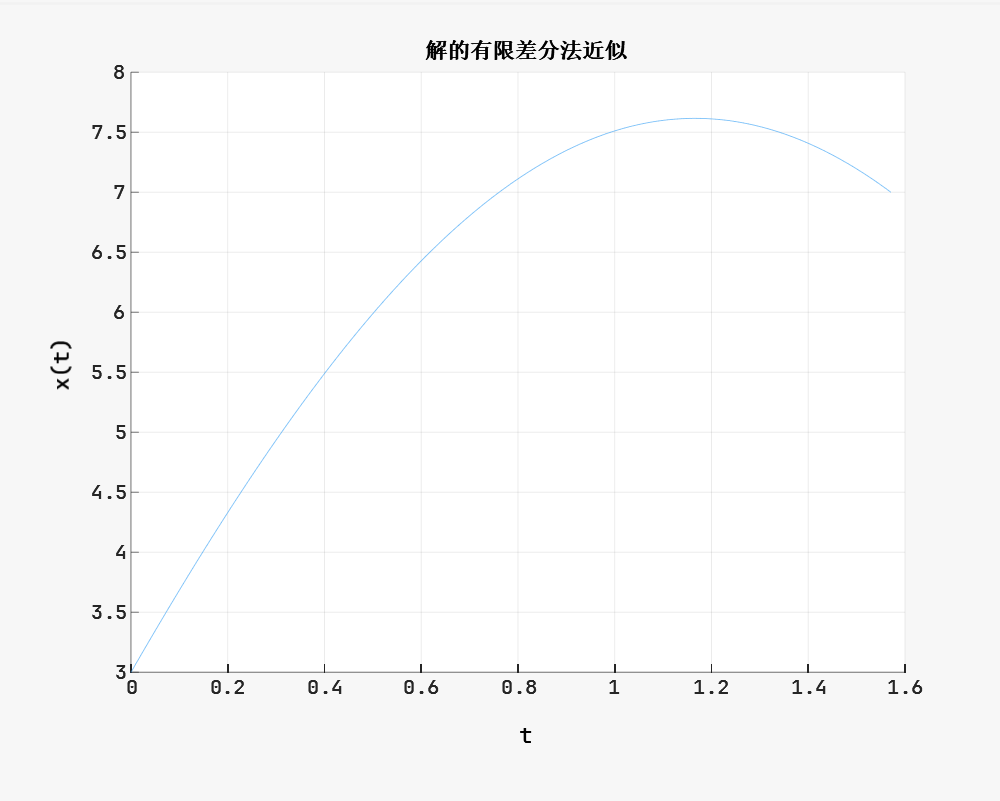
\includegraphics[width=\linewidth]{figure/f1.png}
	\end{subfigure}
	\hspace{0.5cm}
	\begin{subfigure}[b]{0.45\textwidth}
		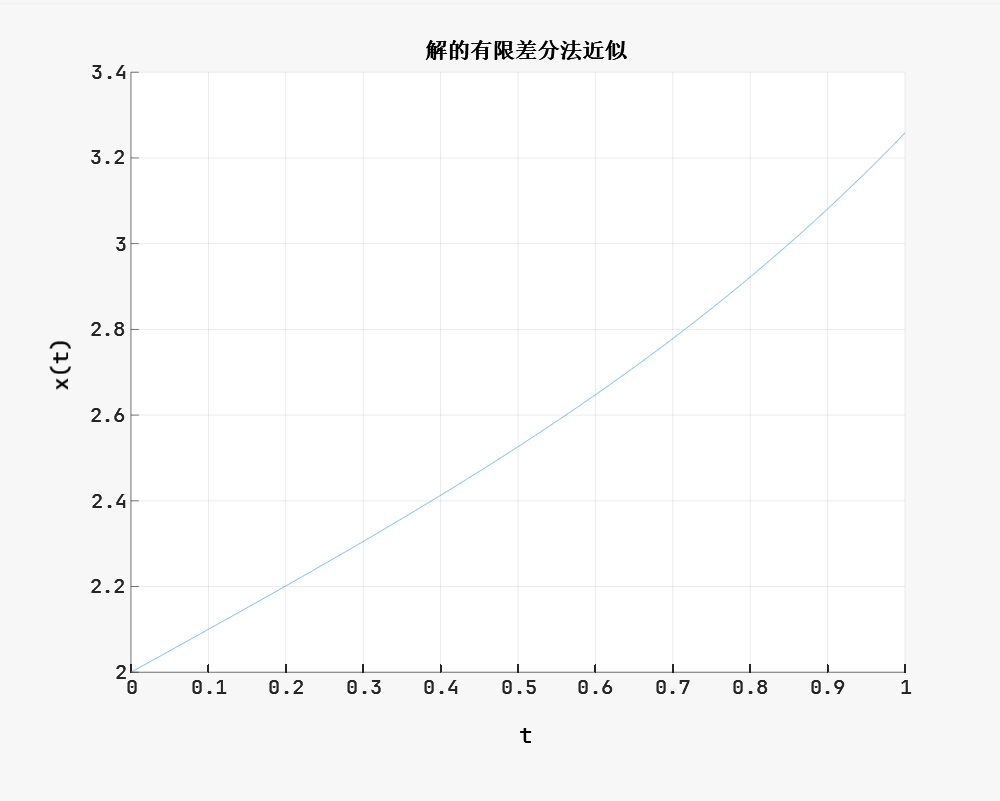
\includegraphics[width=\linewidth]{figure/f2.png}
	\end{subfigure}
	\caption{问题 1 和问题 2 的数值解图像}
\end{figure}

\subsection{误差和收敛阶}
\begin{figure}[ht]
	\centering
	\begin{subfigure}[b]{0.45\textwidth}
		\centering
		\begin{tabular}{ccc}
		\toprule
		$N$ & 最大误差 & 收敛阶 \\
		\midrule
		10  & $5.7324\mathrm{e}{-03}$ & --     \\
		20  & $1.4288\mathrm{e}{-03}$ & 2.0043 \\
		40  & $3.5749\mathrm{e}{-04}$ & 1.9988 \\
		80  & $8.9356\mathrm{e}{-05}$ & 2.0003 \\
		160 & $2.2341\mathrm{e}{-05}$ & 1.9999 \\
		\bottomrule
		\end{tabular}
	\end{subfigure}
	\hspace{0.5cm}
	\begin{subfigure}[b]{0.45\textwidth}
		\centering
		\begin{tabular}{ccc}
		\toprule
		$N$ & 最大误差 & 收敛阶 \\
		\midrule
		10  & $2.9584\mathrm{e}{-04}$ & --     \\
		20  & $7.3917\mathrm{e}{-05}$ & 2.0008 \\
		40  & $1.8496\mathrm{e}{-05}$ & 1.9987 \\
		80  & $4.6244\mathrm{e}{-06}$ & 1.9999 \\
		160 & $1.1562\mathrm{e}{-06}$ & 1.9999 \\
		\bottomrule
		\end{tabular}
	\end{subfigure}
	\caption{问题 1 和问题 2 的误差与收敛阶对比}
\end{figure}

结果表明差分格式在这两个问题中都具有良好的二阶收敛性, 与理论分析一致.

\section{结论}

本实验验证了有限差分法在求解边值问题时的有效性, 数值误差与收敛阶表明算法达到了预期的二阶精度.

未来可考虑推广至变系数问题或非线性边值问题, 进一步验证算法的通用性与稳定性.

\end{document}
